\documentclass{standalone}
\usepackage{tikz,amsmath}
\tikzset{ block/.style = {draw, fill=white, very thick, rectangle, minimum height=1cm, minimum width=2cm},}
\tikzset{sum/.style= {draw, fill=white, very thick, circle, node distance=1cm},}
\begin{document}
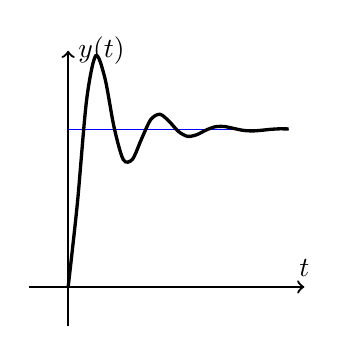
\begin{tikzpicture}[scale=2]
    \draw[->,thick](-0.25,0)--(1.5,0)node[above]{$t$};
    \draw[->,thick](0,-0.25)--(0, 1.5)node[right]{$y(t)$};

    \draw[-, blue](0,1)--(1.4,1);
    \draw[-, very thick]plot[smooth, domain=0:1.4](\x,{1-e^(-4*\x)*cos(16*\x r)});
\end{tikzpicture}
\end{document}